\documentclass[crop,class=article]{standalone}
%----------------------------Preamble-------------------------------%
\usepackage{tikz}                       % Drawing/graphing tools.
\usetikzlibrary{arrows.meta}            % Latex and Stealth arrows.
%--------------------------Main Document----------------------------%
\begin{document}
    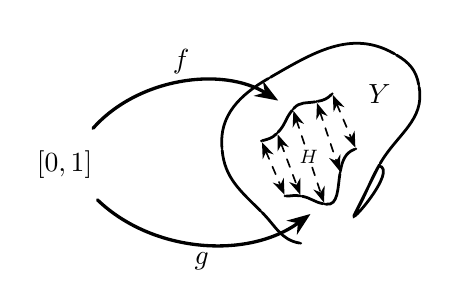
\begin{tikzpicture}[%
        line width=1pt,
        line cap=round,
        >={Stealth[black]},
        every edge/.style={draw=black,very thick},
        smalldot/.style={
            circle,
            fill=black,
            inner sep=0pt,
            outer sep=0
        },
        dashcurve/.style={
            draw=black,
            dashed,
            <->
        }
    ]
        \begin{scope}[every node/.style=smalldot]
            % Set points for upper curve.
            \node at (2.5,1.3) (a0) {};
            \node at (2.7,1.4) (b0) {};
            \node at (2.9,1.7) (c0) {};
            \node at (3.2,1.8) (d0) {};
            \node at (3.4,1.9) (e0) {};

            % Set points for lower curve.
            \node at (2.8,0.6) (a1) {};
            \node at (3,0.6) (b1) {};
            \node at (3.3,0.5) (c1) {};
            \node at (3.5,0.9) (d1) {};
            \node at (3.7,1.2) (e1) {};

            % Points for the outer blob.
            \node at (3,0) (a2) {};
            \node at (2.5,0.4) (b2) {};
            \node at (2,1.2) (c2) {};
            \node at (2.6,2.1) (d2) {};
            \node at (4.2, 2.4) (e2) {};
            \node at (4.5, 2) (f2) {};
            \node at (4,1) (g2) {};
            \node at (3.7,0.4) (h2) {};
        \end{scope}

        % Nodes labelling the domain and co-domain.
        \node at (0,1) (i) {$[0,1]$};
        \node at (4,1.9) (i1) {$Y$};

        % Draw upper curve.
        \draw (a0) to [out=15,in=-135] (b0)
                   to [out=45,in=-130] (c0)
                   to [out=50,in=-170] (d0)
                   to [out=10,in=-135] (e0);

        % Draw lower curve.
        \draw (a1) to [out=0,in=170] (b1)
                   to [out=-10,in=170] (c1)
                   to [out=-10,in=-100] (d1)
                   to [out=80,in=-160] (e1);

        \begin{scope}[%
            every path/.style=dashcurve,
            every edge/.style=semithick
        ]
            % Draw dashed lines connecting curves.
            \path (a0) edge (a1);
            \path (b0) edge (b1);
            \path (c0) edge
                node[inner sep=0pt,outer sep=0pt,fill=white]
                {\scriptsize{\textit{H}}} (c1);
            \path (d0) edge (d1);
            \path (e0) edge (e1);
        \end{scope}

        % Draw curve defining the blob.
        \draw (a2) to [out=170,in=-45] (b2)
                   to [out=135,in=-85] (c2)
                   to [out=95,in=-150] (d2)
                   to [out=30,in=150] (e2)
                   to [out=-30,in=100] (f2)
                   to [out=-80,in=60] (g2)
                   to [out=-120,in=60] (h2)
                   to [out=-120,in=-10] cycle;


        % Draw curves representing maps f and g.
        \path[shorten >=0.2cm,shorten <=0.2cm,->]
            (i) edge[bend left=40]
            node[above] {$f$} (c0);
        \path[shorten >=0.2cm,shorten <=0.2cm,->]
            (i) edge[bend right=40]
            node[below] {$g$} (c1);
    \end{tikzpicture}
\end{document}